\chapter {Zespołowe przedsięwzięcie inżynierskie. Android - kadrowanie}
\section{Członkowie zespołu z określeniem funkcji}
\begin{itemize}
\item [1.] Damian Pulit - lider projektu, programista usług,
\item [2.] Paweł Bodziony - zaopatrujący w potrzebne materiały i informacje,
\item [3.] Patryk Kubisz - zaopatrujący w potrzebne materiały i informacje. 
\end{itemize}
\section {Uzasadnienie potrzeby realizacji projektu}
Projekt realizowany jest w celu stworzenia aplikacji, która zostanie wdrożona do wirtualnego dziekanatu.
Dodanie nowej funkcji do wirtualnego dziekanatu ma usprawnić rekrutację na studia oraz dodawanie zdjęć.
\section {Zakres projektu}
W projekcie zostanie wykonana aplikacja na system android, w której znajdzie się opcja kadrowania i przycinania zdjęć portretowych. W zakres projektu wchodzą następujące elementy, tj. opcje, z których będzie można korzystać podczas używania aplikacji kadrowania na telefonie posiadającym system operacyjny Android:
\begin{itemize}
\item wykonanie lub wczytanie istniejącego już zdjęcia,
\item skadrowanie go za pomocą wpisania proporcji (np. proporcje zdjęcia do legitymacji studenckiej 4:5), bądź wpisania rozmiaru w pikselach (np. rozmiar zdjęcia do legitymacji studenckiej 236x295 px.,
\item zapisanie zdjęcia.
\end{itemize}
\newpage

\section{Grupy docelowe}
Aplikacja kadrowanie przeznaczona jest dla osób, które potrzebują szybkiego skadrowania zdjęcia do wymaganych rozmiarów. Aplikacja zawiera kadrowanie w sposób dowolny, a także za pomocą proporcji i rozmiarów podanych przez użytkownika. Aplikacja ta posiada tylko podstawowe opcje kadrowania, dlatego przeznaczona jest dla początkujących użytkowników, oraz dla takich, którzy cenią sobie prostotę i konkret. Skadrowanie i zapisanie zdjęcia trwa dosłownie kilkanaście sekund. Nie wymaga rejestracji, nie posiada reklam, jest w stu procentach darmowa. Dodatkowo projekt ten będzie miał znaczący wpływ na usprawnienie oraz przyspieszenie przyjmowania kandydatów na studia. Zniknie problem ze zdjęciami w złym wymiarze oddawanymi przez kandydatów.

\section{Plan realizacji projektu}
\begin{itemize} \itemsep1pt \parskip0pt \parsep0pt
\item [1.] \textit{12.10.2016} - Wyszukanie w Internecie kodu źródłowego aplikacji kadrującej.
\item [2.] \textit{12.10.2016} - Zebranie informacji na temat co aplikacja powinna posiadać.
\item [3.] \textit{12.10.2016} - Wyszukanie odpowiedniego środowiska programistycznego.
\item [4.] \textit{19.10.2016} - Instalacja środowiska oraz potrzebnych składników do wirtualizacji telefonu z systemem Android na komputerze. 
\item [5.] \textit{26.10.2016} - Przygotowanie interfejsu aplikacji, tj. ekran powitalny aplikacji oraz ekran z funkcją wczytywania zdjęć.
\item [6.] \textit{09.11.2016} - Dodanie do aplikacji funkcji wczytywania i przycinania zdjęć.
\item [7.] \textit{16.11.2016} - Dodanie do aplikacji funkcji zapisywania zdjęć.
\item [8.] \textit{23.11.2016} - Dodanie opcji wyboru dodatkowych proporcji do kadrowania zdjęć.
\item [9.] \textit{30.11.2016} - Dodanie opcji wyboru kadrowania zdjęć za pomocą wpisywania rozmiaru w pikselach.
\item [10.] \textit{14.12.2016} - Skonfigurowanie przycisku menu w oknie startowym.
\item [11.] \textit{14.12.2016} - Dodanie funkcji wyświetlania bieżących ustawień aplikacji (proporcje, rozdzielczość).
\item [12.] \textit{21.12.2016} - Dodanie przycisku odpowiedzialnego za otwarcie galerii po skadrowaniu zdjęcia. 
\item [13.] \textit{21.12.2016} - Stworzenie strony internetowej do pobrania aplikacji. 
\end{itemize}

\section{Organizacja zarządzania projektem}
Osobami odpowiedzialnymi za tworzenie projektu są: Damian Pulit, Paweł \\ Bodziony i Patryk Kubisz. 

Do obowiązków lidera należy:
\begin{itemize} \itemsep1pt \parskip0pt \parsep0pt
\item wyznaczanie obowiązków dla poszczególnych członków zespołu,
\item nadzorowanie pracy poszczególnych członków zespołu,
\item planowanie, a następnie kierowanie realizacją projektu według określonych działań i terminów, 
\item kontrolowanie przebiegu projektu i ewentualne jego korygowanie,
\item motywowanie zespołu,
\item konsultowanie wymagań dotyczących projektu ze zleceniodawcą.
\end{itemize}
$\qquad$ Do obowiązków członków zespołu należą:
\begin{itemize}\itemsep1pt \parskip0pt \parsep0pt
\item wykonywanie poleceń lidera,
\item wykonywanie zgodnie z harmonogramem poszczególnych etapów projektu.
\end{itemize}
\section{Zasoby niezbędne do realizacji projektu}
\begin{itemize}
\item [a)] \textbf{ludzkie}: umiejętności programistyczne w języku Java, umiejętność pracy ze środowiskiem Eclipse, nabycie wiedzy związanej z tworzeniem aplikacji na system Android,
\item [b)] \textbf{materialne}: telefon z system z Android, kompilator Eclipse, jednostka stacjonarna lub mobilna PC, dostęp do Internetu.
\end{itemize}


\chapter {Damian Pulit}
\section{Zadanie projektowe}
\noindent\textbf{Rodzaj zadania:}  Wyszukanie w Internecie kodu źródłowego aplikacji kadrującej.\\

\noindent\textbf{Data rozpoczęcia:} 2016-10-12\\

\noindent\textbf{Data zakończenia:} 2016-10-19\\
\\

 Kadrowanie jest to proces usuwania fragmentów fotografii w celu skupienia uwagi na jego części lub poprawienia kompozycji. Do kadrowania i prostowania zdjęć w programie Photoshop służy narzędzie Kadrowanie. Działanie narzędzia Kadrowanie nie powoduje modyfikacji danych obrazu. Wykadrowany obraz można zachować w celu późniejszej zmiany granic kadrowania.\\

W internecie znajduje się wiele aplikacji do kadrowania zdjęć. Autorzy niektórych z nich udostępnili ich kody źródłowe, z których każdy może skorzystać.\\

Znalazłem 3 przykładowe programy wraz z udostępnionym kodem źródłowym:

\begin{itemize}
\item \textbf{Android-Crop} użytkownika \textbf{jdamc}\\
\textbf{Link:} https://github.com/jdamcd/android-crop\\

\noindent \textbf{Funkcje:}\\
- Projekt GRADLE\\
- Nowoczesny UI\\
- Siatka podczas kadrowania\\
- Ustawienie proporcji\\
- Kompatybilność wsteczna z SDK 10\\
- Przykładowa konfiguracja\\
- Przykładowy projekt\\
\begin{figure}[h!]
\centering
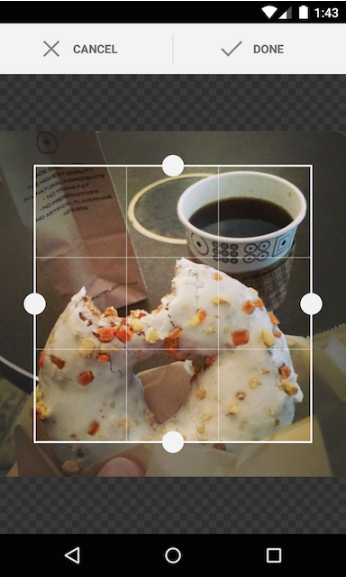
\includegraphics[width=0.25\linewidth]{fig/d1}
\caption{Android-Crop / jdamc}
\label{fig:d1}
\end{figure}\\

\item \textbf{Android-Image-Cropper} użytkownika \textbf{ArthurHub}\\
\textbf{Link:} https://github.com/ArthurHub/Android-Image-Cropper\\

\noindent \textbf{Funkcje:}\\
- Ustawienie skadrowanego zdjęcia jak Bitmapa\\
- Obracanie zdjęcia podczas kadrowania\\
- Ustawienie proporcji\\
- Auto zoom podczas kadrowania\\
- Auto obracanie zdjęcia podczas wczytywania\\
- Kompatybilność z API 10\\
- Siatka podczas kadrowania\\
- Intuicyjność interfejsu\\
\begin{figure}[h!]
\centering
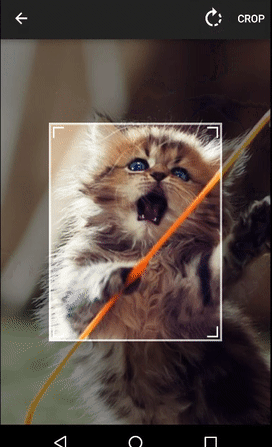
\includegraphics[width=0.25\linewidth]{fig/d2}
\caption{Android-Image-Cropper / ArthurHub}
\label{fig:d2}
\end{figure}\\

\item \textbf{Cropper} użytkownika \textbf{edmodo}\\
\textbf{Link:} https://github.com/edmodo/cropper\\

\noindent \textbf{Funkcje:}\\
- Siatka podczas kadrowania\\
- Ustawienie proporcji\\
\begin{figure}[h!]
\centering
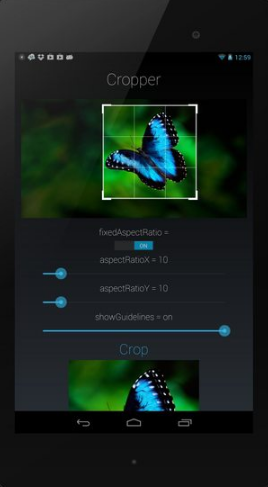
\includegraphics[width=0.25\linewidth]{fig/d3}
\caption{Cropper / edmodo}
\label{fig:d3}
\end{figure}
\end{itemize}

Wybraliśmy program \textbf{Android-Image-Cropper} autorstwa \textbf{ArthurHub} ze względu na ilość funkcji które posiada oraz intuicyjność i prostotę interfejsu.

\section{Zadanie projektowe}
\noindent\textbf{Rodzaj zadania:}  Przygotowanie interfejsu aplikacji.\\

\noindent\textbf{Data rozpoczęcia:} 2016-10-19\\

\noindent\textbf{Data zakończenia:} 2016-10-26\\
\\


\begin{verbatim}
<android.support.v4.widget.DrawerLayout
    xmlns:app="http://schemas.android.com/apk/res-auto"
    android:id="@+id/drawer_layout"
    xmlns:android="http://schemas.android.com/apk/res/android"
    xmlns:tools="http://schemas.android.com/tools"
    android:layout_width="match_parent"
    android:layout_height="match_parent"
    tools:context="com.theartofdev.edmodo.cropper.sample.MainActivity">
    \end{verbatim}
    \begin{center}
    \centering\underline{\textbf{Wysuwane menu}}
    \end{center}
    \begin{verbatim}
    <ScrollView
        android:id="@+id/navigation_drawer"
        android:layout_width="@dimen/navigation_drawer_width"
        android:layout_height="match_parent"
        android:layout_gravity="start"
        android:background="#dfdfdf"
        android:orientation="vertical">

        <LinearLayout
            android:layout_width="@dimen/navigation_drawer_width"
            android:layout_height="wrap_content"
            android:layout_gravity="start"
            android:background="#dfdfdf"
            android:orientation="vertical"
            android:padding="12dp">
\end{verbatim}
\begin{center}
\underline{\textbf{Opcja: Wczytaj zdjęcie}}
\end{center}
\begin{verbatim}
            <TextView
                android:id="@+id/drawer_option_load"
                style="@style/Cropper.Widget.Drawer.Option.TextView"
                android:onClick="onDrawerOptionClicked"
                android:text="@string/main_drawer_load"
                android:textColor="@android:color/black"
                android:textColorHighlight="@android:color/darker_gray"
                 />

        </LinearLayout>
    </ScrollView>

</android.support.v4.widget.DrawerLayout>

\end{verbatim}

\chapter {Paweł Bodziony}
\section{Zadanie projektowe}
\noindent\textbf{Rodzaj zadania:} Wyszukanie odpowiedniego środowiska programistycznego. \\

\noindent\textbf{Data rozpoczęcia:} 2016-10-12\\

\noindent\textbf{Data zakończenia:} 2016-10-19\\


\textbf{Zintegrowane środowisko programistyczne (ang. Integrated Development Environment, IDE)} – aplikacja lub zespół aplikacji (środowisko) służących do tworzenia, modyfikowania, testowania i konserwacji oprogramowania.
\\

Aplikacje będące zintegrowanymi środowiskami programistycznymi charakteryzują się tym, że udostępniają złożoną, wieloraką funkcjonalność obejmującą edycję kodu źródłowego, kompilowanie kodu źródłowego, tworzenie zasobów programu (tzn. formatek / ekranów / okien dialogowych, menu, raportów, elementów graficznych takich jak ikony, obrazy itp.), tworzenie baz danych, komponentów i innych.
\\

\textbf{Przy wyborze odpowiedniego środowiska programistycznego kierowałem się tym aby dane środowisko obsługiwało język Java w którym będzie pisana aplikacja, oraz żeby dane środowisko miało możliwość emulowania telefonu z systemem android do szybkiego testowania aplikacji. Wyselekcjonowane zostały dwa  najbardziej odpowiednie środowiska, którymi były Eclipse oraz Android Studio.}
\\

Oprogramowanie Android studio oferuje podobne możliwości co środowisko Eclipse z zainstalowaną wtyczką ADT, jednak jest ono znacznie prostsze i bardziej intuicyjne w szczególności dla początkujących programistów. Przejęło ono wszystkie najlepsze rozwiązania znane użytkownikom IntelliJ, oferując narzędzie zoptymalizowane w dużym stopniu do wygodnej pracy z kodem źródłowym. Decydując się na korzystanie z Android Studio użytkownik otrzymuje środowisko programistyczne z przejrzystym i konfigurowalnym interfejsem graficznym, nie wspominając o funkcji kolorowania składni czy mechanizmie zakładek, pozwalającym na pracę z wieloma plikami jednocześnie.

\textbf{W ostateczności wybór padł na Android Studio, główną cechą która zdecydowała była możliwość wirtualizacji telefonu z systemem android w przeciwieństwie do środowiska Eclipse.}
\\

W środowisku Android Studio z pewnością odnajdą się zarówno początkujący programiści, jak również ci bardziej zaawansowani. Twórcy postarali się, aby poza samym narzędziem do pisania kodu developerzy znaleźli w nim także inne, przydatne podczas codziennej pracy funkcje i narzędzia. W tym miejscu wspomnieć należy m.in. o debugerze, liście ToDo, pozwalającej organizować zadania do wykonania w obrębie danego projektu czy mechanizmowi wirtualnych urządzeń do testowania tworzonych aplikacji.




\section{Zadanie projektowe}
\noindent\textbf{Rodzaj zadania:} Instalacja środowiska oraz potrzebnych składników do wirtualizacji telefonu z systemem Android na komputerze. \\

\noindent\textbf{Data rozpoczęcia:} 2016-10-19\\

\noindent\textbf{Data zakończenia:} 2016-10-26\\


Do rozpoczęcia projektu programiście niezbędne są różne zasoby, między innymi takie jak środowisko programistyczne, które zostało wcześniej wybrane oraz zainstalowane i odpowiednio skonfigurowane na komputerze roboczym.
\\

Android Studio to środowisko programistyczne (IDE) stworzone przez Google na bazie IntelliJ, które kierowane jest do developerów aplikacji na Androida. Pozwala ono wygodnie projektować, tworzyć i debugować własne programy na najpopularniejszą obecnie platformę systemową dla urządzeń mobilnych.
\\

Środowisko programistyczne Android Studio możemy pobrać bezpłatnie ze strony pod adresem: \textit{https://developer.android.com/studio/index.html}. Środowisko jest przystosowane do różnych systemów operacyjnych, takich jak Linux, Mac OS, oraz Windows. Wybrałem wersję na system Windows, gdyż taki system został zainstalowany na komputerze roboczym.
\\


\textbf{Na poniższych zrzutach ekranu została przedstawiona instalacja środowiska programistycznego Android studio.}

\begin{figure}[h!]
\centering
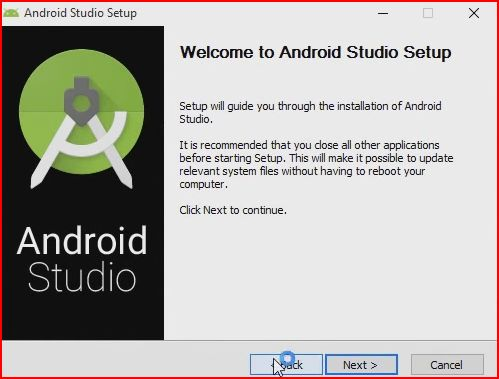
\includegraphics[width=0.5\linewidth]{fig/i1}
\caption{Ekran początkowy instalacji}
\label{fig:11}
\end{figure}

\begin{figure}[h!]
\centering
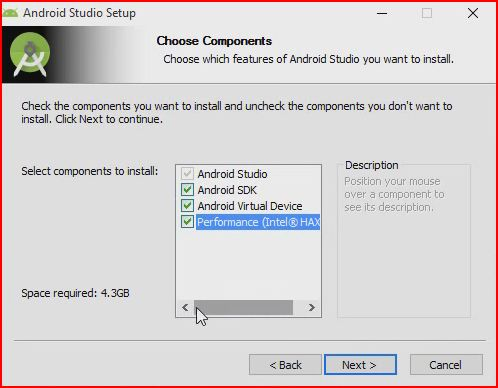
\includegraphics[width=0.5\linewidth]{fig/i2}
\caption{Wybór potrzebnych składników instalacji}
\label{fig:12}
\end{figure}

\begin{figure}[h!]
\centering
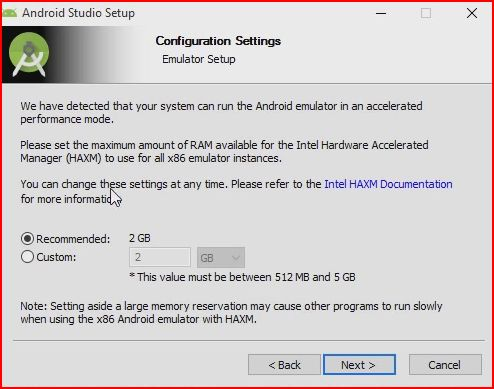
\includegraphics[width=0.5\linewidth]{fig/i3}
\caption{Wybór rekomendowanej ilości pamięci RAM w celu przyspieszenia działania Android Studio}
\label{fig:13}
\end{figure}

\begin{figure}[h!]
\centering
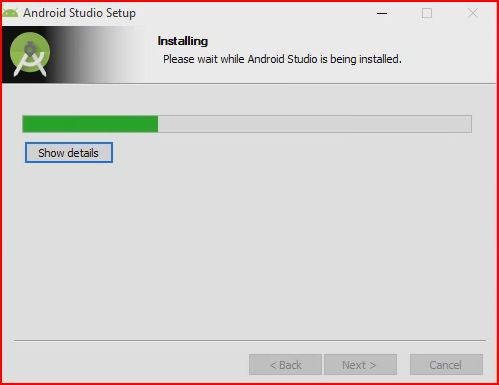
\includegraphics[width=0.5\linewidth]{fig/i4}
\caption{Proces instalacji}
\label{fig:14}
\end{figure}

\begin{figure}[h!]
\centering
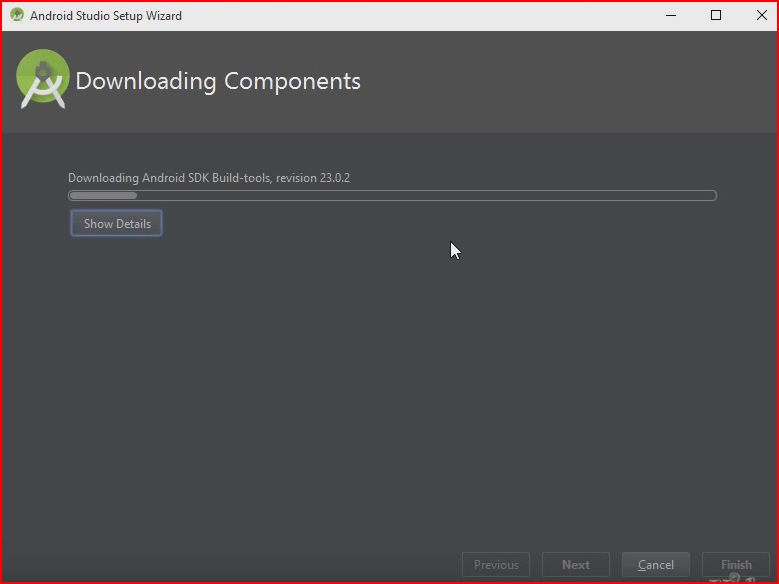
\includegraphics[width=0.5\linewidth]{fig/i5}
\caption{Pobieranie wybranych komponentów programu}
\label{fig:15}
\end{figure}

\begin{figure}[h!]
\centering
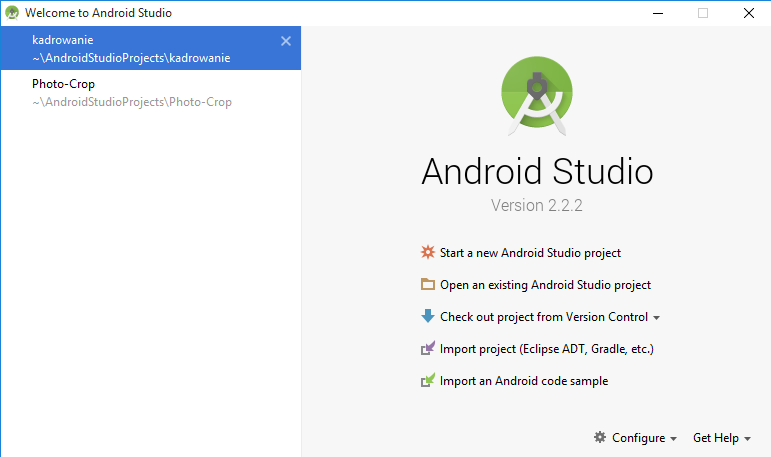
\includegraphics[width=0.7\linewidth]{fig/i6}
\caption{Ekran powitalny Android Studio}
\label{fig:16}
\end{figure}




\chapter {Patryk Kubisz}
\section{Zadanie projektowe}

\noindent\textbf{Rodzaj zadania:} Zebranie informacji na temat co aplikacja powinna posiadać.\\

\noindent\textbf{Data rozpoczęcia:} 2016-10-12\\

\noindent\textbf{Data zakończenia:} 2016-10-19\\

\noindent\textbf{Wstęp}\\

Aplikacja kadrowanie została stworzona z myślą o szybkim i wygodnym kadrowaniu zdjęć. W naszych planach było stworzenie aplikacji, która pozwoli na szybkie skadrowanie zdjęcia za pomocą proporcji lub podanych rozmiarów w formacie px. W naszym zamyśle aplikacja nie miała posiadać trudnych do pojęcia opcji dla zwykłego użytkownika, czyli nie miała to być aplikacja "wszystko w jednym". Aplikacja nie posiada  tworzenia kolaży i rysowania, czy udostępniania zdjęć. Nie posiada filtrów, przycinania oraz tego typu funkcji. Jej podstawową funkcją to wczytanie - skadrowanie - zapisanie. Poniżej zostają zamieszczone poszczególne informacje na temat wdrażanych rozwiązań w procesie tworzenia aplikacji:
\begin{itemize}
\item [1.] \textbf{Intuicyjny interfejs} czyli interakcja człowieka z aplikacją, interfejs użytkownika nazywany jest przestrzenią w której dochodzi do interakcji. Celem tej interakcji jest umożliwienie skutecznego operowania i kontroli nad aplikacją przez człowieka, podczas gdy aplikacja dostarcza zwrotnych informacji ułatwiając operatorowi podejmowanie decyzji. Zależało nam na tym aby interfejs był łatwy w obsłudze, aby nie trzeba było poświęcać czasu na szukanie poszczególnych opcji w aplikacji. Do tej aplikacji potrzebny jest przejrzysty i intuicyjny interfejs.
\newpage
\item [2.] \textbf{Wdrożone funkcje} zostały wybrane spośród tych najbardziej niezbędnych do szybkiego skadrowania zdjęcia. Do podstawowych funkcji jakie zostały wdrożone w aplikacji należą:
\begin{itemize}
\item \textit{\textbf{aparat}} daje możliwość wykonania zdjęcia prosto z poziomu aplikacji. Nie wymaga się od użytkownika, aby korzystał z aparatu przed uruchomieniem aplikacji.
\item \textit{\textbf{galeria}} przenosi użytkownika w miejsce gdzie są zapisane wcześniej zdjęcia od razu z poziomu aplikacji. Można edytować zapisane wcześniej zdjęcia, bez uprzedniego wchodzenia w galerię.
\item \textit{\textbf{proporcje dowolne}} umożliwiają użytkownikowi ustawienie dowolnych proporcji za pomocą przesuwania palcem po zdjęciu. Po ustawieniu proporcji aplikacja domyślnie rozpozna ustawione przez użytkownika proporcje i zamieści je w górnej części ekranu w celu przedstawienia użytkownikowi w jakich proporcjach przyciął zdjęcie. 
\item \textit{\textbf{proporcje ustawiane}} umożliwiają użytkownikowi wybór proporcji spośród podanych. Wybieralne proporcje mieszczą się w przedziale od 1:10 do 10:1. Na przykład, gdy użytkownik chce skadrować zdjęcie do legitymacji wybiera proporcje 4:5 przy maksymalnej rozdzielczości (tj. rozdzielczości wykonanego wcześniej zdjęcia).
\item \textit{\textbf{ustawiany rozmiar}} umożliwia użytkownikowi wybór rozmiaru zdjęcia w pikselach, na przykład, gdy użytkownik chce skadrować zdjęcie do legitymacji za pomocą rozmiaru, wybiera 236x295 px. Są to proporcje 4:5, lecz rozmiar zdjęcia nie jest maksymalizowany, jak w przypadku kadrowania za pomocą proporcji, lecz według ustawień użytkownika.
\item \textit{\textbf{zapis zdjęcia}} do galerii. Po zapisaniu zdjęcia można bezpośrednio przejść do galerii, aby zobaczyć skadrowane zdjęcie. Można go także ponownie skadrować i nadpisać, lecz konsekwencją może być utracona jakość zdjęcia. W przypadku edycji zdjęcia zalecane jest, aby otworzyć na nowo zdjęcie, które chcieliśmy skadrować. 
\end{itemize}
\end{itemize}

\section{Zadanie projektowe}
\noindent\textbf{Rodzaj zadania:}  Przygotowanie interfejsu aplikacji.\\

\noindent\textbf{Data rozpoczęcia:} 2016-10-19\\

\noindent\textbf{Data zakończenia:} 2016-10-26\\
\\


\begin{verbatim}
<android.support.v4.widget.DrawerLayout
    xmlns:app="http://schemas.android.com/apk/res-auto"
    android:id="@+id/drawer_layout"
    xmlns:android="http://schemas.android.com/apk/res/android"
    xmlns:tools="http://schemas.android.com/tools"
    android:layout_width="match_parent"
    android:layout_height="match_parent"
    tools:context="com.theartofdev.edmodo.cropper.sample.MainActivity">
    \end{verbatim}
    \begin{center}
    \centering\underline{\textbf{Wysuwane menu}}
    \end{center}
    \begin{verbatim}
    <ScrollView
        android:id="@+id/navigation_drawer"
        android:layout_width="@dimen/navigation_drawer_width"
        android:layout_height="match_parent"
        android:layout_gravity="start"
        android:background="#dfdfdf"
        android:orientation="vertical">

        <LinearLayout
            android:layout_width="@dimen/navigation_drawer_width"
            android:layout_height="wrap_content"
            android:layout_gravity="start"
            android:background="#dfdfdf"
            android:orientation="vertical"
            android:padding="12dp">
\end{verbatim}
\begin{center}
\underline{\textbf{Opcja: Wczytaj zdjęcie}}
\end{center}
\begin{verbatim}
            <TextView
                android:id="@+id/drawer_option_load"
                style="@style/Cropper.Widget.Drawer.Option.TextView"
                android:onClick="onDrawerOptionClicked"
                android:text="@string/main_drawer_load"
                android:textColor="@android:color/black"
                android:textColorHighlight="@android:color/darker_gray"
                 />

        </LinearLayout>
    </ScrollView>

</android.support.v4.widget.DrawerLayout>

\end{verbatim}

\chapter{Zadania wspólne}

\section{Zadanie projektowe}
\noindent\textbf{Rodzaj zadania:}  Zaprogramowanie w aplikacji funkcji wczytywania i przycinania zdjęć.\\

\noindent\textbf{Data rozpoczęcia:} 2016-10-26\\

\noindent\textbf{Data zakończenia:} 2016-11-09\\

\begin{center}
\underline{\textbf{Funkcja wczytywania zdjęć:}}
\end{center}

\begin{verbatim}
@Override
    @SuppressLint("NewApi")
    protected void onActivityResult
    (int requestCode, int resultCode, Intent data) {
        super.onActivityResult
        (requestCode, resultCode, data);

        if (requestCode == 
        CropImage.PICK_IMAGE_CHOOSER_REQUEST_CODE && resultCode
         == AppCompatActivity.RESULT_OK) {
            Uri imageUri = 
            CropImage.getPickImageResultUri(this, data);
            lub.setVisibility(View.INVISIBLE);
            btnOne.setVisibility(View.INVISIBLE);
            boolean requirePermissions = false;
            if (CropImage.isReadExternalStoragePermissionsRequired
            (this, imageUri)) {

                requirePermissions = true;
                mCropImageUri = imageUri;
                requestPermissions(new String[]
                {Manifest.permission.READ_EXTERNAL_STORAGE},
                 CropImage.PICK_IMAGE_PERMISSIONS_REQUEST_CODE);
            } else {

                mCurrentFragment.setImageUri(imageUri);
            }
        }
    }

    @Override
    public void onRequestPermissionsResult(int requestCode, 
    String permissions[], int[] grantResults) {
        if (requestCode == 
        CropImage.CAMERA_CAPTURE_PERMISSIONS_REQUEST_CODE)
         {
            if (grantResults.length > 0 && grantResults[0] == 
            PackageManager.PERMISSION_GRANTED) {
                CropImage.startPickImageActivity(this);
            } else {
                Toast.makeText(this, "Cancelling, 
                required permissions are not granted", 
                Toast.LENGTH_LONG).show();
            }
        }
        if (requestCode == CropImage.PICK_IMAGE_PERMISSIONS_REQUEST_CODE) {
            if (mCropImageUri != null && grantResults.length > 
            0 && grantResults[0] == PackageManager.PERMISSION_GRANTED) {
                mCurrentFragment.setImageUri(mCropImageUri);
            } else {
                Toast.makeText(this, 
                "Cancelling, required permissions are not granted", 
                Toast.LENGTH_LONG).show();
            }
        }
    }
\end{verbatim}
\begin{center}
\underline{\textbf{Funkcja kadrowania zdjęć:}}
\end{center}
\begin{verbatim}
private void handleCropResult(CropImageView.CropResult result) {
        if (result.getError() == null) {
            Intent intent = new Intent(getActivity(), CropResultActivity.class);
            intent.putExtra("SAMPLE_SIZE", result.getSampleSize());
            if (result.getUri() != null) {
                intent.putExtra("URI", result.getUri());
            } else {
                CropResultActivity.mImage = mCropImageView.getCropShape()
                 == CropImageView.CropShape.OVAL
                        ? CropImage.toOvalBitmap(result.getBitmap())
                        : result.getBitmap();
            }

            startActivity(intent);
        } else {
            Log.e("AIC", "Failed to crop image", result.getError());
            Toast.makeText(getActivity(), "Image crop failed: " + 
            result.getError().getMessage(), Toast.LENGTH_LONG).show();
        }
    }
\end{verbatim}
